\documentclass[tikz,border=3mm]{standalone}
\usepackage{times}
\usepackage{amsmath}
\usetikzlibrary{arrows.meta,positioning,shapes.geometric,fit,calc}

\definecolor{kbblue}{RGB}{46,98,164}
\definecolor{queryorange}{RGB}{217,120,42}
\definecolor{execgreen}{RGB}{69,145,94}
\definecolor{softblue}{RGB}{232,240,250}
\definecolor{softorange}{RGB}{252,239,225}
\definecolor{softgreen}{RGB}{231,244,235}
\definecolor{softgray}{RGB}{245,246,248}
\definecolor{linegray}{RGB}{72,78,88}

\begin{document}
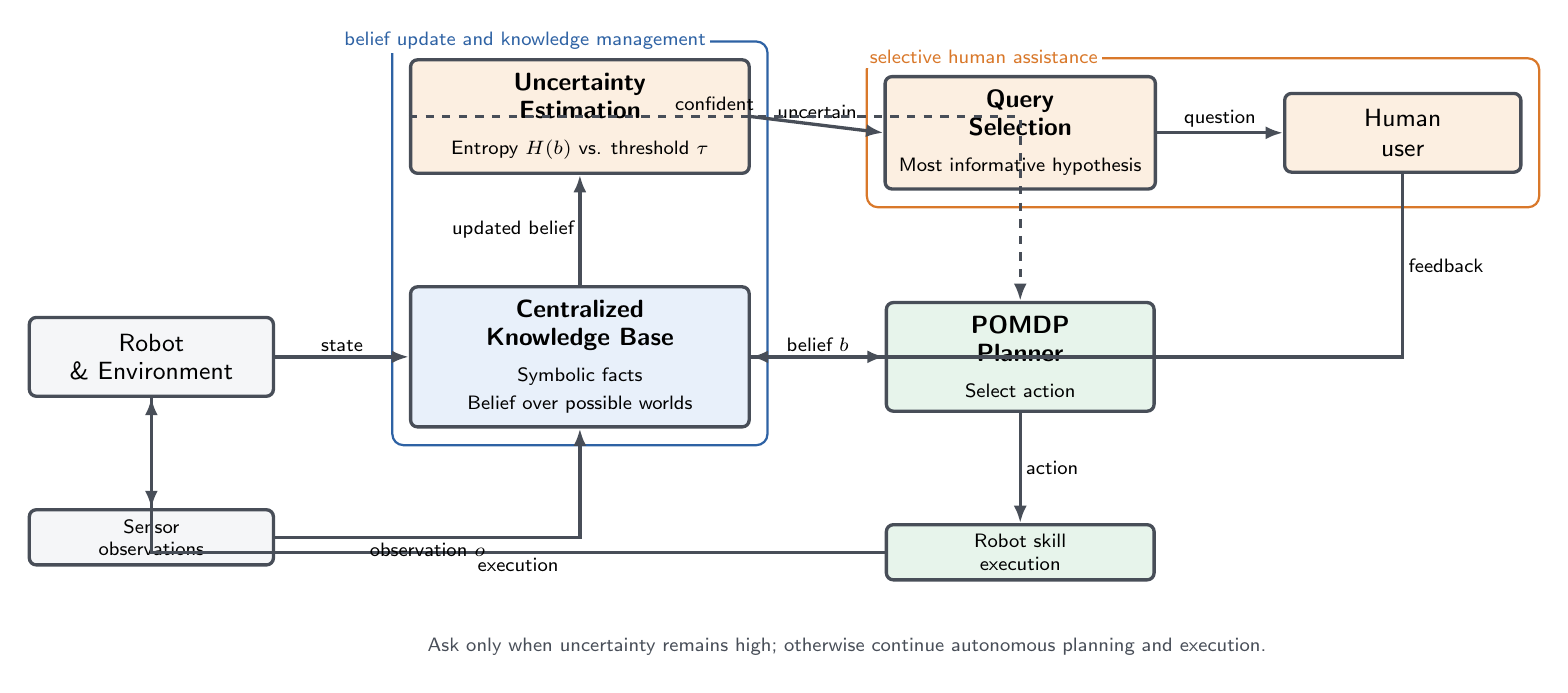
\begin{tikzpicture}[
    font=\sffamily\small,
    node distance=10mm and 12mm,
    block/.style={
        rectangle,
        rounded corners=2.5pt,
        draw=linegray,
        very thick,
        align=center,
        minimum height=10mm,
        inner xsep=5pt,
        inner ysep=5pt
    },
    smallblock/.style={
        block,
        font=\sffamily\scriptsize,
        minimum height=7mm,
        inner xsep=4pt,
        inner ysep=3pt
    },
    arrow/.style={-{Latex[length=2.2mm]}, very thick, draw=linegray},
    dashedarrow/.style={-{Latex[length=2.2mm]}, very thick, dashed, draw=linegray},
    label/.style={font=\sffamily\scriptsize, inner sep=1.5pt}
]

% Main modules
\node[block, fill=softgray, minimum width=31mm] (env)
    {Robot\\[-1pt]\& Environment};

\node[block, fill=softblue, minimum width=43mm, right=17mm of env] (kb)
    {\textbf{Centralized}\\[-1pt]\textbf{Knowledge Base}\\[2pt]
     \scriptsize Symbolic facts\\[-1pt]
     \scriptsize Belief over possible worlds};

\node[block, fill=softgreen, minimum width=34mm, right=17mm of kb] (planner)
    {\textbf{POMDP}\\[-1pt]\textbf{Planner}\\[2pt]
     \scriptsize Select action};

\node[smallblock, fill=softgreen, below=14mm of planner, minimum width=34mm] (skill)
    {Robot skill\\execution};

\node[smallblock, fill=softgray, below=14mm of env, minimum width=31mm] (obs)
    {Sensor\\observations};

\node[block, fill=softorange, above=14mm of kb, minimum width=43mm] (uncert)
    {\textbf{Uncertainty}\\[-1pt]\textbf{Estimation}\\[2pt]
     \scriptsize Entropy $H(b)$ vs. threshold $\tau$};

\node[block, fill=softorange, above=14mm of planner, minimum width=34mm] (query)
    {\textbf{Query}\\[-1pt]\textbf{Selection}\\[2pt]
     \scriptsize Most informative hypothesis};

\node[block, fill=softorange, right=16mm of query, minimum width=30mm] (user)
    {Human\\user};

% Group labels
\node[
    draw=kbblue,
    rounded corners=4pt,
    line width=0.8pt,
    inner sep=6pt,
    fit=(kb) (uncert)
] (beliefgroup) {};
\node[label, text=kbblue, fill=white] at ($(beliefgroup.north west)+(17mm,0)$)
    {belief update and knowledge management};

\node[
    draw=queryorange,
    rounded corners=4pt,
    line width=0.8pt,
    inner sep=6pt,
    fit=(query) (user)
] (querygroup) {};
\node[label, text=queryorange, fill=white] at ($(querygroup.north west)+(15mm,0)$)
    {selective human assistance};

% Main loop
\draw[arrow] (env) -- node[label, above] {state} (kb);
\draw[arrow] (kb) -- node[label, above] {belief $b$} (planner);
\draw[arrow] (planner) -- node[label, right] {action} (skill);
\draw[arrow] (skill.west) -| node[label, below,pos=0.25] {execution} (env.south);
\draw[arrow] (env.south) -- (obs.north);
\draw[arrow] (obs.east) -| node[label, below,pos=0.25] {observation $o$} (kb.south);

% Uncertainty and query path
\draw[arrow] (kb.north) -- node[label, left] {updated belief} (uncert.south);
\draw[arrow] (uncert.east) -- node[label, above] {uncertain} (query.west);
\draw[arrow] (query.east) -- node[label, above] {question} (user.west);
\draw[arrow] (user.south) |- node[label, right,pos=0.25] {feedback} (kb.east);

% Autonomous path
\draw[dashedarrow] (uncert.west) -| node[label, above,pos=0.25] {confident} (planner.north);

% Bottom note
\node[
    align=center,
    font=\sffamily\scriptsize,
    text=linegray,
    below=6mm of skill,
    xshift=-22mm
] (note) {Ask only when uncertainty remains high; otherwise continue autonomous planning and execution.};

\end{tikzpicture}
\end{document}
